\documentclass[12pt]{report}
\usepackage{amsmath}
\usepackage{amsfonts}
\usepackage{amssymb}
\usepackage{graphicx}
\usepackage{tikz}
\usetikzlibrary{shapes,arrows}
\usepackage{geometry}
\usepackage{enumitem}
\usepackage{amsthm}
\usepackage{mathtools}
\usepackage[many]{tcolorbox}
\usepackage{algorithm}
\usepackage{algpseudocode}



\def\bN{{\mathbb N}}
\def\bZ{{\mathbb Z}}
\def\bQ{{\mathbb\bf Q}}
\def\cA{{\mathcal A}}
\def\cC{{\mathcal C}}
\def\cE{{\mathcal E}}
\def\cG{{\mathcal G}}
\def\cH{{\mathcal H}}
\def\cI{{\mathcal I}}
\def\cM{{\mathcal M}}
\def\cO{{\mathcal O}}
\def\cU{{\mathcal U}}
\def\b0{{\underline{0}}}
\def\lra{\longrightarrow}
\def\Lra{\Leftrightarrow}
\def\Ra{\Rightarrow}
\def\lla{\longleftarrow}
\def\la{\leftarrow}
\def\ra{\rightarrow}
\def\wt{\widetilde}
\def\ol{\overline}
\def\tz{\c{t}}
\def\Tz{\c{T}}
\def\sh{\c{s}}
\def\Sh{\c{S}}
\def\ua{\u{a}}
\def\uA{\u{A}}
\def\aa{\^{a}}
\def\AA{\^{A}}
\def\ii{\^{i}}
\def\II{\^{I}}
\def\cart{\times}
\def\pzt{\textbf{p}$_{zt}$}
\def\ci{\mathcal{I}}
\def\bR{\mathbb{R}}
\def\vv{\textbf{v}}
\DeclareMathOperator*{\argmin}{argmin} 

\geometry{
	a4paper,
	total={160mm,257mm},
	left=30mm,
	right=20mm,
	top=20mm,
	bottom=20mm,
}

\graphicspath{ {images/} }

\begin{document}
	
\begin{titlepage}
	
	\begin{center}
		\begin{large}
			Universitatea ``Alexandru Ioan Cuza" din Ia\sh i\\
			Facultatea de Informatic\ua\\
		\end{large}
	\end{center}
	
	\vspace{40mm}
	
	\begin{center}
		
\includegraphics{fii.png}
	\end{center}
	
	\vspace{15mm}
	
	\begin{center}
		\begin{Large}
			LUCRARE DE LICEN\Tz \uA
		\end{Large}
		\\
		\
		\\
		\
		\
		
		\begin{Huge}
			\textbf{Multilinear Maps over Ideal Lattices}
		\end{Huge}
		
		\
		
		propus\ua \space de
		
	\end{center}
	
	\vspace{40mm}
	
	\textbf{Student:} Ciprian B\ua etu
	
	\textbf{Coordonator \sh tiin\tz ific:} Prof. Dr. Ferucio Lauren\tz iu \Tz iplea
	\\
	\
	\\
	\
	
	
	\vfill
	
	\begin{center}
		\textbf{Sesiunea:} iunie - iulie
		
		2017
	\end{center}
	
\end{titlepage}
\newpage

\begin{titlepage}
	
	\begin{center}
		Universitatea ``Alexandru Ioan Cuza" din Ia\sh i\\
		Facultatea de Informatic\ua\\
	\end{center}
	
	\vspace{80mm}
	
	\begin{center}
		\begin{Huge}
			\textbf{Multilinear Maps over Ideal Lattices}
		\end{Huge}
	\end{center}
	
	\vspace{60mm}
	
	\textbf{Student:} Ciprian B\ua etu
	
	\textbf{Coordonator \sh tiin\tz ific:} Prof. Dr. Ferucio Lauren\tz iu \Tz iplea
	
	\vfill
	
	\begin{center}
		\textbf{Sesiunea:} iunie - iulie
		
		2017
	\end{center}
	
\end{titlepage}
\newpage

\

\pagenumbering{arabic}

\vspace{10mm}
\begin{large}
	\begin{center}
		DECLARA\Tz IE PRIVIND ORIGINALITATE \Sh I RESPECTAREA DREPTURILOR DE AUTOR
	\end{center}
\end{large}

\vspace{20mm}

Prin prezenta declar c\ua \space Lucrarea de licen\tz \ua \space cu titlul "Multilinear Maps over Ideal Lattices" este scris{\ua} de mine \sh i nu a mai fost prezentat{\ua}  niciodat{\ua} la o alt{\ua} facultate sau institu\tz ie de \ii nv\ua \tz \ua m\aa nt superior din \tz ar{\ua} sau str\ua in\ua tate. De asemenea, declar c{\ua} toate sursele utilizate, inclusiv cele preluate de pe Internet, sunt indicate \ii n lucrare, cu respectarea regulilor de evitare a plagiatului:

\begin{itemize}
	\item toate fragmentele de text reproduse exact, chiar \sh i în traducere proprie din alt{\ua} limbă, sunt scrise între ghilimele \sh i de\tz in referin\tz a precis{\ua} a sursei;
	\item reformularea \ii n cuvinte proprii a textelor scrise de către al\tz i autori de\tz ine referin\tz a precis\ua ;
	\item codul surs\ua , imaginile etc. preluate din proiecte open-source sau alte surse sunt utilizate cu respectarea drepturilor de autor \sh i de\tz in referin\tz e precise; 
	\item rezumarea ideilor altor autori precizeaz{\ua} referin\tz a precis{\ua} la textul original.
	
\end{itemize}

\vspace{10mm}

Ia\sh i,
\

24 iunie 2017
\

\begin{flushright}
	Absolvent,
	\\
	
	B\ua etu Ciprian
	\\
	\
	\
	
	\line(1,0){150}
	\
	
	(semn\ua tura \ii n original)
\end{flushright}

\newpage

\

\vspace{20mm}
\begin{large}
	\begin{center}
		DECLARA\Tz IE DE CONSIM\Tz \uA M\AA NT
	\end{center}
\end{large}

\vspace{30mm}

Prin prezenta declar c{\ua} sunt de acord ca Lucrarea de licen\tz{\ua} cu titlul "Multilinear Maps over Ideal Lattices", codul surs{\ua} al programelor \sh i celelalte con\tz inuturi (grafice, multimedia, date de test etc.) care \ii nso\tz esc aceast{\ua} lucrare s{\ua} fie utilizate \ii n cadrul \mbox{Facult\ua \tz ii} de Informatic\ua.
\\

De asemenea, sunt de acord ca Facultatea de Informatic{\ua} de la Universitatea „Alexandru Ioan Cuza” din Ia\sh i s{\ua} utilizeze, modifice, reproduc{\ua} \sh i s{\ua} distribuie \ii n scopuri necomerciale programele-calculator, format executabil \sh i surs\ua, realizate de mine \ii n cadrul prezentei lucr\ua ri de licen\tz \ua.

\vspace{20mm}

Ia\sh i,
\

24 iunie 2017
\\
\

\begin{flushright}
	Absolvent,
	\\
	
	B\ua etu Ciprian
	\\
	\
	\
	
	\line(1,0){150}
	\
	
	(semn\ua tura \ii n original)
\end{flushright}
\newpage


\tableofcontents{}
\chapter{Introduction}


\space Usually, cryptographic primitives are constructed under the assumption that several problems are intractable, i.e. there exist no polynomial-running time algorithm to solve them. Vercauteren \cite{Ver13} realized an extensive research regarding the intractable problems that are most used in cryptography, such as integer factoring, discrete logarithm, computational Diffie-Hellman, shortest vector problem and many others.\\

In the last ten years, bilinear maps proved to be very useful in cryptography. Making use of the interesting properties of such maps, cryptographers managed to construct schemes for one-round three-party key exchange \cite{Jou00}, identity based encryption \cite{BoF01} and many other applications. After the moment that bilinear maps proved to be undoubtedly  useful, researchers have tried to generalize the concept. Thus, multilinear maps were defined and the search for their applications has begun. Boneh and Silverberg \cite{BoS02} showed that symmetric multilinear maps can be used to realize a one-round multi-party key exchange scheme but, after their attempts to construct such maps failed, they drew the conclusion that "such maps might have to either come from outside the realm of algebraic geometry, or occur as 'unnatural' computable maps arising from geometry."\\

Garg, Gentry and Halevi \cite{GGH13} proposed a construction based on lattices that approximate the multilinear maps in hard-discrete-logarithm groups. Using this candidate, they could construct an application to multipartite Diffie-Hellman key exchange scheme and also the first construction of Attribute-Based Encryption for general circuits \cite{GGH+13a}. A short period after the aforementioned candidate was proposed, Coron, Lepoint and Tibouchi \cite{CLT13} created a similar construction, based on integers instead of lattices.\\

However, these construction proved to be susceptible to attacks, and a devastating zeroizing attack for the integer construction is presented thoroughly in \cite{CKC+15}. Numerous fixing tentatives of these schemes were designed, but for each of them there was found at least another attack. Therefore currently, new methods of constructing multilinear maps and Graded Encoding Schemes still constitute an open field, very interesting for cryptographers. 
\newpage

\section{Contribution}

This work represents a survey over the bilinear and multilinear maps and their applications. Furthermore, in this paper is presented the concept of Graded Encoding Scheme, a modality of approximating multilinear maps. The core of the paper is represented by the review of the lattice-based construction, designed by Garg, Gentry and Halevi in \cite{GGH13}. 

\section{Organization}

The paper is divised into 5 sections. First one - introduction bla-bla. In the second section, bla bla bla ... etc etc.
\chapter{Multilinear Maps and Graded Encoding Systems}

In this chapter, multilinear maps are defined and also, the particular case of bilinear maps is discussed, along with results concerning self-bilinear applications. Thereafter, \textit{Graded Encoding Schemes} are defined, as an approximate to multilinear maps. \\

\textit{Observation:} Regarding the multilinear applications and Graded Encoding Systems schemes, and also for the lattice-based candidate designed in \cite{GGH13}, the paper encompasses one subsection of efficient procedures, and another one of hardness assumptions. The reader should be aware of this detail and realize the analogy and differences of the mentioned schemes.


\section{Bilinear Maps}
As stated before, bilinear maps are a specific case of multilinear maps. They proved to be a highly useful tool in cryptography, with many applications, such as: tripartite protocol \cite{Jou00}, identity based encryption \cite{BoF01} and Attribute-based encryption scheme for monotone boolean formulas \cite{TiD14}. In this section, bilinear maps are only defined, while next section presents a relationship between self-bilinear maps and multilinear maps. \\

\textbf{Definition 1.} (Bilinear Map \cite{BCM16}). \textit{Given the cyclic groups $G$ and $G_t$ (written additively) of the same order $p$, a (symmetric) map $e:G \cart G \ra G_t$ is said to be bilinear if the following properties hold:
\begin{enumerate}
	\item \textbf{(Bi-linearity)}\space  $e({g_1}^{x_1}, {g_2}^{x_2}) = e(g_1,g_2)^{x_1x_2},$ for any $x_1,x_2 \in \bZ_p$ and any $g_1, g_2 \in G$;
	\item  \textbf{(Non-degeneracy)} \space If $g_1, g_2\in G$ are generators of $G$, then $e(g_1, g_2)$ is a generator of $G_t$;
	\item \textbf{(Efficient computability)} There exists a polynomially-bounded algorithm to compute $e(g_1,g_2)$, for any $g_1,g_2 \in G$.
\end{enumerate} 
}

\section{Cryptographic Multilinear Maps}
\textbf{Definition 2.} (Multilinear Maps \cite{Rot13}). \textit{ Let $k \geq 2$ be an integer number and $G_1, G_2,...,G_k, G_T$ be $k + 1$ cyclic groups (written additively), of same order $p$. Then, a $k-$multilinear map is a mapping $e:G_1\cart...\cart G_k \ra G_T$, with the following properties:
	\begin{enumerate}
		\item \textbf{(Linearity)} For every $g_1\in G_1, ..., g_k \in G_k$, every $i\in \{1,2,..,k\}$ and every $\alpha\in \bZ_p$, it holds that:
\begin{align*}
			e(g_1,...,\alpha \cdot g_i, ..,g_k) = \alpha \cdot e(g_1,...,g_k))
\end{align*}
		\item \textbf{(Non-degeneracy)} If $g_1\in G_1, ..., g_k \in G_k$ are generators of their respective groups, then $e(g_1,...,g_k)$ is a generator of $G_T$.
	\end{enumerate}
}

\subsection{From Self-Bilinear to Multilinear Maps}

\textbf{Definition 3.} \textit{A self-bilinear map is a bilinear map where the domain and target groups are the same.} \\

\textbf{Proposition 1.} \textit{Let $G$ be a cyclic group of order $p$ and $e:G\cart G\ra G$ be a self-bilinear map. Therefore, a $k-$multilinear map $e_k:G^k \ra G$ can be constructed from $e$, for any $k \geq 2$.}\\

\textbf{\textit{Proof.}} The proof is realized by induction. First, for the base case $k = 2$, it is trivial to observe that $e$ itself is a 2-liniar map. Then, suppose that an $n-$multilinear map $e_n:G^n\ra G$ can be constructed starting from $e$, and it can be easily shown that a $(n+1)$-multilinear map $e_{n+1}:G^{n+1}\ra G$ can be constructed, as follows:
\begin{align*}
	e_{n+1}(g_1,..,g_n, g_{n+1}) = e(e_n(g_1,.., g_n), g_{n+1}), \forall g_1, .., g_{n+1} \in G.
\end{align*}
Indeed, from the fact that $e_n$ is multilinear it follows that, for any $g_1\in G_1, ..., g_n \in G_n$, any $i\in \{1,..,n\}$ and any $\alpha \in \bZ_p$,  $e_n(g_1,...,\alpha \cdot g_i, ..,g_n) = \alpha \cdot e_n(g_1,...,g_n))$. Using the bilinearity of $e$, it results that $e_{n+1}$ respects the \textbf{linearity} condition.\\
Let $g_1, ...,g_n$ be generators of $G$. Then, using the fact that $e_{n}$ is $n-$multilinear, it follows that $e_n(g_1,..,g_n)$ is also a generator of $G$. Corroborating the last result with the non-degeneracy property of $e$, it ensues that $e_{n+1}$ respects \textbf{non-degeneracy} condition, from which the conclusion that $e_{n+1}$ is a $(n+1)$-multilinear map can be drawn. \qed\\

However, Cheon and Lee \cite{ChL09} proved that self-bilinear maps on prime order groups do not exist, except that the computational Diffie-Hellman problem is easy. That is the main motivation of \cite{BCM16}, which analyzes the existence of self-bilinear maps on groups of composite order.

\subsection{Efficient Procedures}

In order to use the cryptographic multilinear applications in a real-world environment, efficient procedures must be designed in order to be evaluated by computers. Therefore, as specified in \cite{GGH13}
a cryptographic multilinear map scheme is a 5-uple $\mathcal{MMP} = $ \textbf{(InstGen, EncTest, add, neg, map)}, as described below:
\begin{enumerate}[label=(\alph*)]
	\item \textbf{Instance Generation.}  A procedure with a "factory" role must exist, in order to instantiate the parameters of the scheme. This procedure is \textbf{InstGen}.
	\begin{itemize}
		\item \textbf{Input:} $\lambda $ - the security parameter and $k \geq 2$ - the multilinearity parameter.
		\item \textbf{Output:} (\textbf{params}, $g_1, .., g_k$), where \textbf{params} = ($G_1, .., G_T, p, e$). Here $G_1,..,G_k,$ $G_T$ represent the groups, $p\in \bZ$ is their order, $e$ is the representation of the multilinear map and $g_i \in \{0, 1\}^*$ is the representation of a generator of $G_i$, for every $i \in \{1,..,k\}$.
	\end{itemize}


	\item \textbf{Element Encoding.} A procedure that decides if a sequence of bits represents an encoding of an element in one of the groups must be defined, and it is named \textbf{EncTest}.
		\begin{itemize}
		\item \textbf{Input:} \textbf{params} - the instance parameters, $i \in \{1,..,k+1\}$ - index of the desired group and $x\in \{0,1\}^*$ - encoding of the tested element.
		\item \textbf{Output:} True, if $x$ is a valid encoding of an element in $G_i$, False otherwise. \textit{Note:} The extension $G_{k+1} = G_T$ is performed.
	\end{itemize}


	\item \textbf{Group addition.} The procedure \textbf{add} simply applies the group operation upon two provided elements representations.
\begin{itemize}
	\item \textbf{Input:} \textbf{params} - the instance parameters, $i \in \{1,..,k+1\}$ - index of the desired group, $x,y$ - representations of elements to be added.
	\item \textbf{Output:} the representation of $x+y \in G_i$.                                     
\end{itemize}


	\item \textbf{Group negation.} The procedure \textbf{neg} returns the inverse representation of the  element provided as parameter.
\begin{itemize}
	\item \textbf{Input:} \textbf{params} - the instance parameters, $i \in \{1,..,k+1\}$ - index of the desired group, $x$ - representation of the element to be negated.
	\item \textbf{Output:} the representation of $-x \in G_i$.                                     
\end{itemize}


	\item \textbf{Map computation.} The procedure \textbf{map} returns the representation of the multilinear mapping over the elements given as parameters.
\begin{itemize}
	\item \textbf{Input:} \textbf{params} - the instance parameters, $x_1\in G_1, .., x_k \in G_k$ - elements in domain groups.
	\item \textbf{Output:} the representation of $e(x_1,..,x_k) \in G_T$.
\end{itemize}
\end{enumerate}

\subsection{Hardness Assumptions}







\chapter{Mathematical Background}

The purpose of this chapter is to remind the reader basic notions regarding algebra and statistics, but also to analyze in detail concepts and algorithms concerning lattices, especially integer lattices. 

\section {Algebra}
The notions of group, cyclic group, ring and polynomial are considered to be previously known by the average reader. More information about the mentioned structures can be found in \cite{HPS08}, chapter 2. For a mathematical perspective over groups and polynomial rings properties, and also for a deep incursion in field extension theory, the reader can explore \cite{BB15}.

\begin{enumerate}
	\item \textbf{Ideals and Quotient Rings.} 
	
	\textbf{Definition 5.} \textit{Let $(R, +, \cdot)$ be a commutative finite ring. An \textbf{ideal} of $R$ is a nonempty set $\ci \subseteq R$ that is closed under addition and $ax=xa \in \ci, \forall x \in \ci, \forall a \in R.$} \\
	
	Let $(R, +, \cdot)$ be a finite ring and $\ci$ be an ideal of $R$. Also, let $"\sim"$ be an equivalence relationship on $R$, defined by $x \sim y \iff \exists a\in \ci $ such that $x = y + a$. The equivalence class of an element $x \in R$ is usually noted with $\hat{x}$, and it represents the set $\{y \in R : y \sim x\}$. The equivalence classes generate a partition of the set $R$, named \textit{quotient set}, and denoted by $R/\ci$. It is known that $(R/\ci, +, \cdot)$ is also a ring, and it is called the \textbf{quotient ring} $R/\ci$.
	
	\textbf{Remark 3.} \textit{An example of a quotient ring is the well-known ring $\bZ_p = \bZ/p\bZ.$}
	
	\item \textbf{Cyclotomic polynomials.}
	
	\textbf{Definition 6 \cite{BB15}.} \textit{Let $n \geq 1$ be an integer and $P_n $ be the set of all the $n^{th}$ primitive roots of unity. Then, the \textbf{$n^{th}$ cyclotomic polynomial} is $\Phi_n = \displaystyle{\prod_{\xi \in P_n}}(X-\xi)$}.
	
	\textbf{Remark 4.} Using the fact that $\Phi_{p^k}(X) = \Phi_p(X^{p^{k-1}})$, for any positive integers $k, p$, with $p-$prime, it can be proved that $\Phi_{2^k}(X) = X^{2^{k-1}} + 1,$ for any integer $k \geq 1$.
	
	\item \textbf{Vector spaces}.
	
	Throughout the paper, vectors and matrices are thickened, e.g. $\textbf{v}$. Also, every vector space is considered to be contained in $R^m$, with $m \geq 1$, integer.\\
	
	\textbf{Definition 7 \cite{HPS08}.} \textit{Let $m$ be a positive integer. A \textbf{vector space} $V$ is a subset of $\bR^m$, such that for every $\alpha_1, \alpha_2 \in \bR$ and every} $\textbf{v}_1, \textbf{v}_2 \in V$, it holds: $\alpha_1 \vv_1 + \alpha_2 \vv_2\in V$.
	
	The lecturer is expected to master the concepts of \textit{linear combination, linear independence, basis, vector orthogonality, basis orthogonality}. For a quick review over the mentioned concepts, visit \cite{HPS08}.\\
	
	The only algorithm regarding vector spaces to be presented in the current paper is the  \textbf{Gram-Schmidt Algorithm}. It receives as input a basis $\{\vv_1, .., \vv_n\}$ of the vector space $V$ and outputs $\{\vv_1^*,..,\vv_n^*\}$ - an orthonormal basis of $V$. The algorithm is presented below:

\begin{tcolorbox}[colframe=black,colback=white,arc=0pt,outer arc=0pt]
	\begin{center}
		\textbf{The Gram-Schmidt Algorithm}
	\end{center}
	\begin{algorithmic}[1]
		\State Set $\vv_1^* = \vv_1$
		\For{$i \la 2$ \textbf{to} $n$}
		\State Compute $\mu_{ij} = \vv_i \cdot \vv_j^*$ $/$ $ ||\vv_j^*||$,  for $1 \leq j < i$
		\State Set $\vv_i^* = \vv_i - \displaystyle{\sum_{j = 1}^{i-1}} \mu_{ij} \vv_j^* $
		\EndFor
	\end{algorithmic}
\end{tcolorbox}

	Intuitively, $\mu_{ij}$ represents the length of the projection of $\vv_i$ over $\vv_j^*$. Therefore, the substraction $\vv_i - \mu_{ij} \vv_j^*$ generate the projection of $\vv_i$ over the orthogonal complement of $\vv_j^*$, which leads to the desired output. 
\end{enumerate}	

\section{Lattices}

\subsection{General Influence}

Lattices have been studied by mathematicians such as Gauss, Lagrange or Minkowski since 18$^{th}$ century, and have been used to prove theorems in number theory and the field extensions. Even though lattices confirmed their significance in mathematics, they were not used in computer science until the 1980s, when Lenstra, Lenstra and Lov\`{a}sz proposed the basis-reduction algorithm \textbf{LLL}. It represented a major breakthrough in cryptography, and was used to break several cryptosystems, such as RSA (in a low exponent setting) and NTRU. \\

Since the proposal of \textbf{LLL} algorithm, lattices became appealing to the world of cryptography. Thus, since then they have been used in the construction of cryptographic schemes, such as Attribute Based Encryption \cite{Boy13}, Fully homomorphic encryption \cite{Gen09} and Graded Encoding Systems \cite{GGH13}.

\subsection{Basic Concepts}

\textbf{Definition 8 (\cite{HPS08}).} \textit{Let $n, m$ be two positive integers and let} $B = \{\vv_1, .., \vv_n\} \subset \bR^m$ \textit{ be a set of linearly independent vectors. The \textbf{lattice} generated by $B$ is the set:}
\begin{center}
	$L$   $  \stackrel{\mathclap{\normalfont\mbox{not.}}}{=} \mathcal{L}(B) = \{a_1\vv_1 + a_2 \vv_2 +... + a_n\vv_n : a_1, a_2, ..,a_n \in \bZ\}$.
\end{center}

\textit{Also, a lattice that contains only vectors with integer coordinates is called an \textbf{integer lattice}}. The \textbf{dual lattice} is denoted by $L^* = \{\textbf{y} \in Span(L) : \forall \textbf{x} \in L, \langle\textbf{x, y}\rangle \in \bZ\}$.


From a visual point of view, the elements of a lattice are structured as a net, with massive holes between the nodes, as it can be noticed in Figure 1.

\textbf{Definition 9 (\cite{HPS08}).} \textit{Let $L$ be a $n$-dimensional lattice and} $B = \{\vv_1,...,\vv_n\}$ \textit{be a basis for the lattice $L$. The \textbf{fundamental domain} for $L$ that is associated with $B$ is:}
\begin{center}
	$\mathcal{F}(\vv_1,...,\vv_n) = \{t_1\vv_1 + ...+ t_n\vv_n : t_i \in [0, 1], \forall i \in \{1,..., n\}\}$.
\end{center}


\begin{center}
	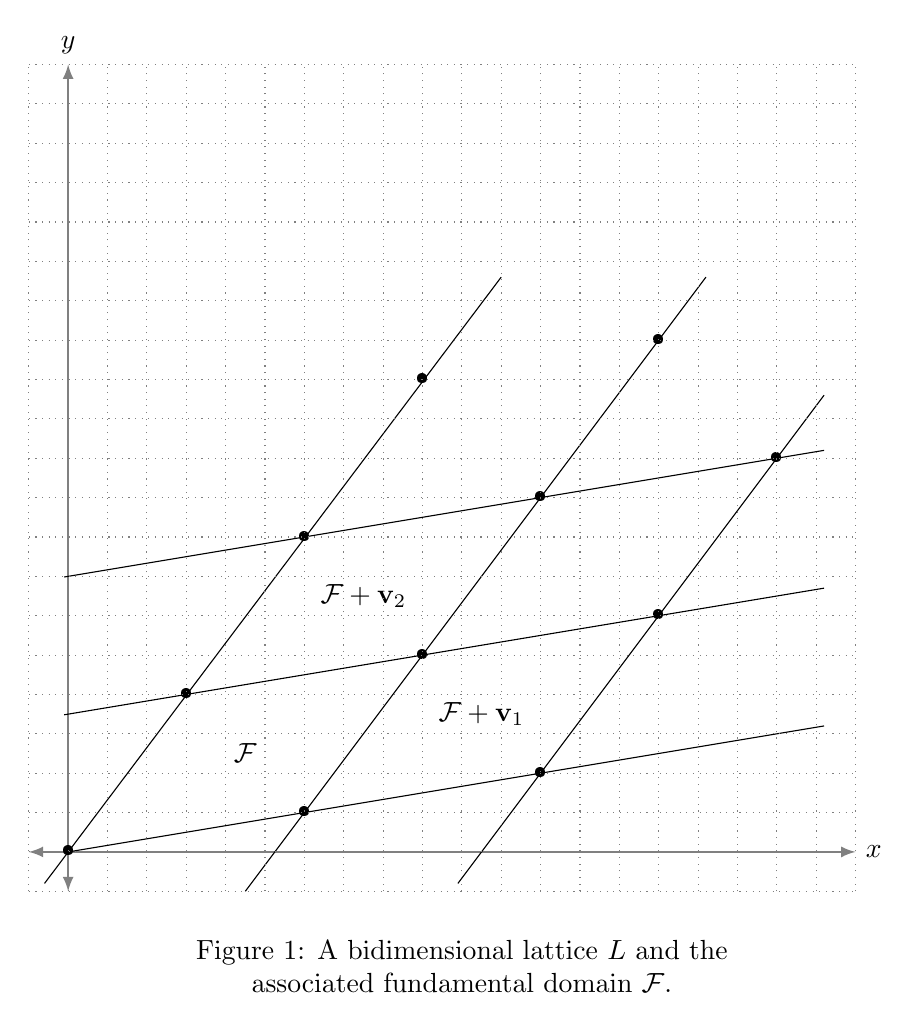
\begin{tikzpicture}[scale = 0.5]
\draw[latex-latex, thick, draw=gray] (-1,0)--(20,0) node [right] {$x$}; 
\draw[latex-latex,thick, draw=gray] (0,-1)--(0,20) node [above] {$y$};

\foreach \Point in {(0, 0), (3, 4), (6,1), (9, 5), (6, 8), (9, 12), (12, 9), (15, 13), (12,2), (15, 6), (18, 10)}{
	\node at \Point {\textbullet};
}

\draw[black] (-0.6, -0.8) -- (11, 14.6);
\draw[black] (4.5, -1) -- (16.2, 14.6);
\draw[black] (9.9, -0.8) -- (19.2, 11.6);

\draw[black] (-0.1, -0.0166) -- (19.2, 3.2);
\draw[black] (-0.1, 3.483333) -- (19.2, 6.7);
\draw[black] (-0.1, 6.983333) -- (19.2, 10.2);


\node [black] at (4.5,2.5) {$\mathcal{F}$};
\node [black] at (10.5,3.5) {$\mathcal{F}+ \vv_1$};
\node [black] at (7.5,6.5) {$\mathcal{F}+ \vv_2$};
\draw [dotted, gray] (-1,-1) grid (20,20);

\node [below=1cm, align=flush center,text width=8cm] at (10, 0)
{
	Figure 1: A bidimensional lattice $L$ and the associated fundamental domain $\mathcal{F}$.
};
\end{tikzpicture}
\end{center}

\textbf{Proposition 2.} \textit{Let $n$ be a positive integer and $L \subset \bR^n$ be a lattice of dimension $n$. Then, for every basis $B$ of $L$, the volume of the fundamental domain associated with it is the same.}\\

\textbf{Definition 10.} \textit{Let $n$ be a positive integer and let $L \subset \bR^n$ be a lattice of dimension $n$. The \textbf{determinant} of $L$ is the volume of any fundamental domain for $L$, and it is denoted by det($L$).}

\subsection{Hard problems}

In order to be able to use lattices in the design of cryptographic schemes, it is required that hard problems related to them to be known. Some of the most important hard problems related to lattices are presented below \cite{HPS08}:

\begin{itemize}
	\item  \textbf{Shortest Vector Problem (SVP).} Let $n$ be a positive integer and $L$ be a lattice of dimension $n$. The problem to find a vector $\vv = \displaystyle{\argmin_{ \textbf{w} \in L \backslash \{\textbf{0}\}}} ||\textbf{w}||$ is referred to as \textbf{SVP}.\\
	
	\item \textbf{Closest Vector Problem (CVP).} Let $n$ be a positive integer and $L$ be a lattice of dimension $n$. Also, let $\textbf{w}$ be a vector in $\bR^n \backslash L$. The problem to find a vector $\vv\in L$ that satisfies $||\textbf{w} - \vv|| = \displaystyle{\min_{ \textbf{u} \in L}} ||\textbf{w} - \textbf{u} || $ is called \textbf{CVP}.\\
	
	\item \textbf{Approximate Shortest Vector Problem (apprSVP).} Let $\psi : \bN \ra \bR$ be a function of one parameter and let $\lambda_1(L) \in L$ be one of the shortest vectors in $L$ (i.e. a solution to \textbf{SVP}). The problem to find a vector $\vv \in L \backslash \{\textbf{0}\}$ such that $||\vv|| \leq \psi(n) \cdot || \lambda_1(L) ||$ is called \textbf{apprSVP}.\\

	\item \textbf{Approximate Closest Vector Problem (apprCVP).} Let $\psi : \bN \ra \bR$ be a function of one parameter, let $\textbf{u} \in \bR^n \backslash L$ be a non-lattice vector and let $\textbf{w}$ be a solution to \textbf{CVP} associated with $\textbf{u}$. The problem to find a vector $\vv \in L$ such that $||\vv - \textbf{u} || \leq \psi(n) \cdot ||\textbf{w} - \textbf{u}||$ is called \textbf{apprCVP}.
\end{itemize}

\textbf{Remark 5. } \textit{\textbf{apprSVP} is known to be hard to solve, even for polynomial approximation functions $\psi$. Also, it is resistant to quantum computing attacks, as opposed to integer factorization problem, which becomes easy in a quantum computing environment, using Schor's algorithm.}

\subsection{Results concerning short vectors}

In order to verify how accurate is the returned solution of an approximation algorithm, it is needed to have an estimate of the desired result. Therefore, an approximative value of the shortest vector length in a lattice is necessary for testing the result of an algorithm solving \textbf{apprSVP}. \\

The current subsection only states the most important results regarding shortest vector length in a lattice. The lecturer who is interested in the proofs of the following results may find them in \cite{HPS08}.\\

\textbf{Definition 11.} \textit{Let $n$ be a positive integer and $L$ be a lattice of dimension $n$. Also, let} $B = \{\vv_1,...,\vv_n\}$ \textit{be a basis of $L$. The \textbf{Hadamard ratio} is defined by:}
\begin{center}
	$\mathcal{H}(B) = \Big(\frac{\text{det}(L)}{||\vv_1|| \cdot ||\vv_2|| \cdot ... \cdot ||\vv_n||} \Big)^{1/n}$.
\end{center}
\textit{The Hadamard ratio is a real number in the interval (0, 1] and it represents a measure of the orthogonality of the basis $B$, with the understanding that the closer the Hadamard ratio is to 1, the more orthogonal are the vectors in $B$.}\\

\textbf{Theorem 1 (Minkowski's Theorem \cite{HPS08}).} \textit{Let $n$ be a positive integer and $L\subset \bR^n$ be a lattice of dimension $n$. If $S \subset \bR^n$ is a symmetric convex set with the property that} $Vol(S) > 2^n \text{det}(L),$ \textit{then $S$ contains a nonzero lattice vector. If $S$ is also a closed set, then it is sufficient to verify that }$Vol(S) \geq 2^n \text{det}(L)$. \\

\textbf{Theorem 2 (Hermite's Theorem \cite{HPS08}).} \textit{Let $n$ be a positive integer. Then, for every lattice $L$ of dimension $n$, there exists a vector} $\vv \in L \backslash\{\textbf{0}\}$ \textit{such that}  $||\vv|| \leq \sqrt{n} \cdot \text{det} (L) ^{1/n}$.\\

\textbf{Remark 6.} \textit{The Hermite's Theorem is a consequence of Minkowski's Theorem, where the set $S$ is considered to be a hypercube in $\bR^n$ centered at \textbf{0}. Considering $S$ to be a hypersphere instead of a hypercube, centered at \textbf{0}, the upper bound in Hermite's theorem is lowered by a factor of $\sqrt{\frac{2}{\pi e}}$}.\\

\textbf{Proposition 3 (\cite{HPS08}).} \textit{Let $n$ be a positive integer and $L\subset \bR^n$ be a lattice of dimension $n$. The \textbf{Gaussian heuristic} affirms that the length of the shortest nonzero vector in $L$ is expected to be} $\sigma(L) = \sqrt{\frac{n}{2\pi e}}\big(\text{det}(L)\big)^{1/n}$.

The vigilant reader may note that the \textit{gaussian expected shortest length} is two times smaller than the upper bound presented in \textit{Remark 6}. \\

\subsection{LLL Algorithm}

The hard problems \textbf{SVP} and \textbf{CVP} may become easy if an orthogonal basis for the lattice is known in advance. It can be quickly verified that a solution to \textbf{SVP} is in fact the shortest vector in the orthogonal basis.\\

The result is usually accurate even for quasi-orthogonal basis, i.e. basis with a Hadamard ratio reasonably close to 1. Babai designed an algorithm that solves \textbf{CVP} in a setting in which a quasi-orthogonal basis is known. \textbf{Babai's Algorithm} receives as input a quasi-orthogonal basis $B = \{\vv_1,...,\vv_n\}$ of the lattice $L \subset \bR^n$ and a vector $\textbf{w} \in \bR^n$. It outputs a vector $\vv\in \bR^n$, solution to \textbf{CVP} problem. The algorithm is presented below, based on \cite{HPS08}:\\


\begin{tcolorbox}[colframe=black,colback=white,arc=0pt,outer arc=0pt]
	\begin{center}
		\textbf{Babai's Algorithm}
	\end{center}
	\begin{algorithmic}[1]
		\State Find $\alpha_1, \alpha_2,...,\alpha_n \in \bR $ such that $\textbf{w} = \alpha_1\vv_1 + \alpha_2\vv_2+...+\alpha_n\vv_n$
		\For{$i \la 12$ \textbf{to} $n$}
		\State Set $\beta_i = \big\lfloor \alpha_i + \frac{1}{2}$\big\rfloor
		\EndFor
		\State $\vv = \beta_1 \vv_1 + \beta_2 \vv_2 +...+\beta_n\vv_n$
	\end{algorithmic}
\end{tcolorbox}
~\\

Therefore, solving \textbf{SVP} or \textbf{CVP} for a lattice $L$ reduces to finding a quasi-orthogonal basis for $L$. The \textbf{LLL} algorithm managed to fill this gap, for lattices of low dimension (i.e. less than 300). Hence, the algorithm had a colossal success among the cryptographers, and it represented the first step to include lattices in the world of cryptography.\\

Presented in \cite{LLL82}, the \textbf{LLL} algorithm was initially conceived to provide a polynomial-time algorithm for factoring polynomials with rational coefficients. Two necessary conditions were formulated for a basis $B = \{\vv_1, ..., \vv_n\}$ in order to be considered \textit{LLL reduced}:

\begin{itemize}
	\item \textbf{Size condition:} $|\mu_{i,j}| =  \frac{|\vv_i \cdot \vv_j^*|}{||\vv_j^*||^2} \leq \frac{1}{2}, \forall$ $ 1 \leq j < i \leq n$;
	
	\item \textbf{Lov\'asz Condition:} $|| \vv_i^* || \geq \big( \frac{3}{4} - \mu_{i,i-1}^2 \big) ||\vv_{i-1}^*||^2, \forall $ $1 < i \leq n$,
\end{itemize}
where $B^* = \{\vv_1^*, ..., \vv_n^*\}$ is the orthogonal basis returned by the \textbf{Gram-Schmidt} algorithm and $\mu_{i,j}$ refers to the constants defined in the same algorithm.\\

\textbf{Proposition 4. (LLL reduced basis apprSVP \cite{HPS08}).} \textit{ Let $n$ be a positive integer and let $L \subset \bR^n$ be a lattice of dimension $n$. For any \textbf{LLL reduced basis}} $B = \{\vv_1,...,\vv_n\}$, \textit{the following property holds:}
\begin{center}
	$||\vv_1|| \leq 2^{(n-1) / 2} \cdot \displaystyle{\min_{\vv \in L \backslash \{\textbf{0}\}} || v||}$.
\end{center}

As it can be easily observed, using the \textbf{LLL} lattice-reduction algorithm leads to solving \textbf{apprSVP} by a factor of $2^{(n-1)/2}$. \\

\textbf{LLL} algorithm is presented below, in the version illustrated by the book of Hoffstein, Pipher and Silverman, \cite{HPS08}. The input of the algorithm is a basis $B = \{\vv_1,\vv_2,...,\vv_n\}$, and the output is the basis $B$, modified as a \textit{LLL reduced basis}: \\

\begin{tcolorbox}[colframe=black,colback=white,arc=0pt,outer arc=0pt]
	\begin{center}
		\textbf{LLL Algorithm}
	\end{center}
	\begin{algorithmic}[1]
		\State Set k = 2
		\State Set $\vv_1^* = \vv_1$
		\While{$k \leq n$}
		\For {$j \la k-1$ \textbf{downto} $1$}
		\State Set $\vv_k = \vv_k - \big\lfloor \mu_{k,j} + \frac{1}{2} \big\rfloor \vv_j$     \Comment \textbf{Size Reduction}
		\EndFor
		
		\If{$||\vv_k^*||^2 \geq \big( \frac{3}{4} - \mu_{k,k-1}^2 \big) ||\vv_{k-1}^*||^2$} \Comment \textbf{Lov\'asz Condition}
		\State Set $k = k + 1$
		\Else 
		\State Swap $\vv_{k-1}$ and $\vv_k$ 
		\State Set $k=\max (k-1, 2)$
		\EndIf
		\EndWhile
	\end{algorithmic}
\end{tcolorbox}
~\\

\textbf{Theorem 3 (LLL Correctness and Running Time \cite{HPS08}).} \textit{Let $n$ be a positive integer, let $L \subset \bR^n$ be a lattice of dimension $n$ and let} $B = \{\vv_1,...,\vv_n\}$ \textit{be a basis for $L$. Then, the \textbf{LLL algorithm}, presented above, returns an \textbf{LLL reduced basis} for $L$, and also it terminates in a finite number of steps.}\\

\textbf{Remark 7.} \textit{The algorithm executes the steps [3]-[13] no more than $\mathcal{O}(n^2 \log n + n^2 \log D)$ times, where} $D = \displaystyle{\max_{\textbf{w} \in B} ||\textbf{w}||}$. \textit{Thus, LLL is a polynomial-time algorithm}.\\

\textbf{LLL} proved its utility in cryptanalysis, its applications covering attacks on the family of knapsack public-key cryptosystems, but also on GGH and NTRU cryptosystems. 

\section{Probabilities and Statistics}

The construction of the Graded Encoding Scheme exposed in \cite{GGH13} requires in-depth results concerning probabilities and statistics, mainly due to the nondeterministic character of the encodings of elements. Therefore, the current section presents the essential results regarding discrete Gaussian distributions over lattices, the sum of discrete Gaussians and the smoothing parameter for a lattice.\\

\begin{enumerate}
	\item \textbf{Gaussian distributions \cite{AGH+12}.} The ellipsoid, continuous $n-$ dimensional Gaussian distribution, with mean {\boldmath$\mu$} and covariance matrix {\boldmath$\Sigma$} is denoted by $\mathcal{N}^n($ {\boldmath$\mu, \Sigma)$}, and has the density function $f(\textbf{x}) = \frac{1}{\sqrt{(2\pi)^k |\Sigma|\cdot}} \exp \big( -\frac{1}{2}$ {\boldmath$(\textbf{x} - \mu)^T \Sigma ^{-1} (\textbf{x} - \mu)$}$\big)$.\\
	
	\textbf{Definition 12.} \textit{ Let $m,n$ be two positive integers, let $S \in \bR^{m\cart n}$ be a rank-$n$ matrix and let {\boldmath$\mu$}$\in\bR^n$ be an $n-$dimensional vector. The \textbf{ellipsoid Gaussian function} over $\bR^n$, centered at {\boldmath$\mu$} and with parameter $S$ is denoted by:}
	\begin{center}
		$\rho_{S, \bm{\mu}}(\textbf{x}) = \exp \big(-\pi (\textbf{x} - \bm{\mu})^T(S^TS)^{-1}(\textbf{x} - \bm{\mu}) \big), \forall \textbf{x}\in \bR^n$.
	\end{center}

	For the particular case $\bm{\mu} = \textbf{0}$, the short version $\rho_S(\cdot)$ is used.\\
	
	\textbf{Definition 13.} \textit{Let $m,n$ be two positive integers, let $S \in \bR^{m\cart n}$ be a rank-$n$ matrix and let $L \subset \bR^n$ be an $n-$dimensional lattice. The \textbf{ellipsoid discrete Gaussian distribution} over $L$, centered at \textbf{0} and with parameter $S$ is:} 
	\begin{center}
		$\mathcal{D}_{L,S}(\textbf{x}) = \frac{\rho_S(\textbf{x})}{\rho_S(L)}, \forall \textbf{x} \in L$,
	\end{center}
\textit{where} $\rho_S(L) = \displaystyle{\sum_{\textbf{x}\in L} \rho_S(\textbf{x})}$.
	
	\item \textbf{Smoothing parameter \cite{MiR04}.} Intuitively, the \textit{smoothing parameter} of a lattice represents a lower bound for the value of the radius of a discrete Gaussian distribution $\mathcal{D}$ with the property: if a noise vector is extracted from $\mathcal{D}$ and is reduced modulo the fundamental domain of the lattice, then the resulted distribution is close to uniform. Formally, the smoothing parameter is defined below:\\
	
	\textbf{Definition 14 (Smoothing parameter \cite{MiR04}).} Let $n$ be a positive integer,  let $L \subset \bR^n$ be an $n-$dimensional lattice and let $\epsilon$ be a positive real number. The \textbf{smoothing parameter} for $L$ and $\epsilon$ is denoted by $\eta_\epsilon(L)$ and represents the smallest $s \in \bR$ such that $\rho_{1/s}(L^* \backslash \{\textbf{0}\}) \leq \epsilon$.

	\textbf{Lemma 1 (\cite{AGH+12}).} Let $m,n$ be two positive integers,  let $L \subset \bR^n$ be an $n-$dimensional lattice, $\epsilon \in (0,1)$ and let $S\in\bR^{m\cart n}$ be a rank-$n$ matrix such that $\sigma_n(S) \geq \eta_\epsilon(L)$. Then, 
	\begin{center}
		$\displaystyle{\Pr_{v \la \mathcal{D}_{L, S}}} \big( ||\vv|| \geq \sigma_1(S) \sqrt{n} \big)\leq \frac{1 + \epsilon}{1 - \epsilon} \cdot 2^{-n}$,
	\end{center}
where $\sigma_1(S), \sigma_n(S)$ denote the largest, respectively the least singular values of $S$.


\end{enumerate}


\chapter{Proposed Encoding Scheme}

Garg, Gentry and Halevi constructed a Graded Encoding Scheme based on ideal lattices, in \cite{GGH13}. Their construction was the first candidate to approximate multilinear maps, therefore had a tremendous impact in the world of cryptography. The current chapter intends to present the system designed by the three aforementioned authors, in an in-depth manner. 

\section{Overview}

To start with, the ring $R$ denotes the cyclotomic polynomial ring $\bZ[X]/(X^n +1)$, for some integer $n$ - power of two. The ring $R$ is often considered to be the lattice $\bZ^n$, because a correspondence between the two structures is obvious. Also, $g \in R$ is a short ring element and $\id = \langle g \rangle$ is the principal ideal generated by $g$. Additionaly, an element $\zz$ is extracted randomly in $R_q$. \\

The elements to be encoded by the scheme are the equivalence classes (or \textbf{cosets}) of the quotient ring $QR = R / \id$, denoted by $\eh$, for some $e \in R$. \\

A level-zero encoding of a coset $\eh$ is a short vector in that coset. The existence of a small vector in any coset is assured by the fact that $g$ is a short element, therefore the basis $B(g) = \{g, Xg,...,X^{n-1}g\}$ has all elements small - only circular permutations of the vector $g$, eventually with a changed sign. Hence, the fundamental domain itself of $B(g)$ is small and because for any $e \in R$, there exists an element $e_g \in \mathcal{F}(B(g))$ such that $e_g \in \eh$, the result follows immediately.\\

For any $i \in \{1,2...,k\}$, the set of all level-$i$ encodings of a coset $\eh$ is $S_i^{\eh} = \big\{ \frac{c}{\zz^i}\in R_q : c \in eh, ||c|| < q^{1/8}\big\}$. The value $||c||$ will be referred to as the \textbf{noise level} of the encoding.\\

\section{Efficient Procedures}

The procedures to be presented are a specific case of the efficient procedures introduced in Subsection 1.4.1. Thus, in this section only the implementation of the mentioned functions will be exposed, as in \cite{GGH13}, with a high-level algorithm exposed in the beginning of every procedure, and the in-depth explanation afterwards. Note that $R$ may be identified by $\bZ^n$, and $R_q$ by $\bZ_q^n$. Also, $K$ denotes the field $\bQ[X]/(X^{n}+1)$.\\

\begin{enumerate}[label=(\alph*)]
	\item \textbf{Instance generation}: (params, \pzt) $\la$ InstGen($1^\lambda, 1^k$).
	
	\begin{tcolorbox}[colframe=black,colback=white,arc=0pt,outer arc=0pt]
		\begin{center}
			\textbf{InstGen($1^\lambda, 1^k$)}
		\end{center}
		\begin{algorithmic}[1]
			\State Choose $g \la \mathcal{D}_{\bZ^n, \sigma}$ (encoding of the generator, element kept \textbf{private}).
			\Statex
			
			\State Choose $\zz\la R_q$ (encoding of a \textbf{private} element, used for encoding elements on level higher than 0).
			\Statex
			
			\State Choose $a \la \mathcal{D}_{\hat{1}, \sigma''}$, then compute a \textbf{public} level-one representation of $\hat{1}$, $\textbf{y} = \big[\frac{\textbf{a}}{\textbf{z}}\big]_q$.
			\Statex
			
			\State Choose $\textbf{b}_i \la \mathcal{D}_{\hat{0}, \sigma'''}, \forall i \in \{1,2,..., m\}$ and compute $\xx_i = \big[\frac{\textbf{b}_i}{\textbf{z}}\big]_q, \forall i \in \{1,2,..., m\}$, \textbf{public} level-one representations of $\hat{0}$. Also, set  $X = (\xx_1 | \xx_2 |...|\xx_m)^T$.
			\Statex
			
			\State Choose $\textbf{h} \la \mathcal{D}_{\bZ^n, \sqrt{q}}$ such that $h \notin \id$, then compute the zero-testing parameter \pzt$=\big[\frac{\textbf{hz}^k}{\textbf{g}}\big]_q$.
			\Statex
			
			\State Choose $s \la \bZ$.
			\Statex
			
			\State \textbf{Output}: params = ($n, q, \textbf{y}, \xx_1,\xx_2,..,\xx_m, s$), \pzt.
		\end{algorithmic}
	\end{tcolorbox}

	\begin{enumerate}[label=\arabic*:]
		\item The uniform extraction of $g$ from the spherical Gaussian distribution $\mathcal{D}_{\bZ^n, \sigma}$, with $\sigma = \sqrt{\lambda n}$, is performed repeatedly, until the following conditions are met:
		
		\begin{itemize}
			\item $||g|| \leq \sigma \sqrt{n}$ and $g$ is invertible in $R_q$;
			\item $g^{-1}$ is a short vector;
			\item $\textbf{N}(g)$ is a prime $\geq 2^{O(n)}$, where $\textbf{N}(g)$ denotes the norm of the ideal $\langle g \rangle$, as defined in \cite{Gar15}, chapter 5.
		\end{itemize}
		
		The last condition implies that $\id = \langle g \rangle$ is a \textbf{prime ideal}. Also, \textbf{Lemma 6.1} from \cite{Gar15} proves that the algorithm above completes in polinomially many trials.
		
		
		\item $\zz$ is chosen uniformly from $R_q$, thus with overwhelming probability is not "small". Using \cite{Gar15} (\textit{Lemma 5.20}), it follows that with overwhelming probability, $\zz$ is invertible in $R_q$.
		
		\item Parameters $\textbf{y}$ and $X$ will show their usefulness during the \textbf{higher-level encoding} procedure. Also, {\pzt} is used as a zero-testing parameter, while $s$ is used as a seed for a strong randomness extractor.\\
	\end{enumerate}


%%%%%%%%%%%%%%%% Finished Instance Generation %%%%%%%%%%%%%%%%%%%%%%%%%

\item \textbf{Sampling level-zero encodings}: $d \la$ \textbf{samp}(params).

	\begin{tcolorbox}[colframe=black,colback=white,arc=0pt,outer arc=0pt]
	\begin{center}
		\textbf{samp}(params)
	\end{center}
	\begin{algorithmic}[1]
		\State Choose \textbf{$d$} $\la \mathcal{D}_{\bZ^n, \sigma'}$.
		\Statex
		\State \textbf{Output}: \textbf{d}.
	\end{algorithmic}
\end{tcolorbox}

	It can be proved that, if $\sigma' \geq \sqrt{\lambda n}||g||$, then the distribution ($\textbf{d}\mod\id$) is statistically close to the uniform distribution over ($\bZ^n \mod \id$). Therefore, the coset to be sampled is close to uniform.
	
	To prove it, firstly it can be stated that, because $g \in \id$, then $\lambda_1(\id) \leq ||g||$. Also, knowing that $\id$ is an ideal of the $(2n)^{th}$ cyclotomic ring, with $n$ a power of two, it follows from \textbf{Proposition 5} that $\lambda_n(L) = \lambda_1(L)$. Corroborating the two results, it results that $\lambda_n(L)\leq ||g||$. Therefore, applying \textbf{Lemma 1}, it follows that:
	
	\begin{center}
		$\eta_{2^{-\lambda}}(\id) \leq \sqrt{\frac{\ln(2n(1 + 2 ^\lambda))}{\pi}} \cdot \lambda_n(L) \leq  \eta_{2^{-\lambda}}(\id) \leq \sqrt{\frac{\ln(2n(1 + 2 ^\lambda))}{\pi}} \cdot ||g|| \leq \sqrt{n\lambda} ||g||$.
	\end{center}

Since $\sigma' \geq \sqrt{\lambda n}||g||$, it is obvious that $\sigma' \geq \eta_{2^{-\lambda}}(\id)$, therefore the proof is complete. \\

Also, the size of \textbf{d} is bounded by $\sigma'\sqrt{n}$, result proved by \textbf{Lemma 2}.\\

%%%%%%%%%%%%%%%% Finished Sampling Procedure %%%%%%%%%%%%%%%%%%%%%%%%%

\item \textbf{Encodings at higher levels:} $\textbf{u}_i \la \text{enc(params,}i, \textbf{d})$.

	\begin{tcolorbox}[colframe=black,colback=white,arc=0pt,outer arc=0pt]
	\begin{center}
		$\text{\textbf{enc}(params,}i, \textbf{d})$
	\end{center}
	\begin{algorithmic}[1]
		\If {$i == 1$}
		\State Choose $\textbf{r}\la \mathcal{D}_{\bZ^n, \sigma^*}$.
		\State Set $\textbf{u}_i = \big[ \frac{\textbf{yd}}{\textbf{z}} + X^T\textbf{r}\big]_q$.
		\Else
		\State Set $\textbf{u}_i = [\textbf{d}\cdot \textbf{y}^i]_q$.
		\State \textbf{Output:} \textbf{u}$_i$.
		\EndIf
	\end{algorithmic}
\end{tcolorbox}

The necessity of publishing a level-one representation of an element is obvious, from the inherent structure of the construction. The "lifting" of a representation, from a lower level to a higher one, may be performed only using another representation of an element, on a higher level.\\

In order to preserve the element to be encoded and to change only the level of encoding, the public element $\textbf{y}$ is an encryption of element $\hat{1}$ - the neutral element at multiplication in $QR$. Also, because $\textbf{y}$ is a level-one encoding, multiplying another element by it results in "lifting" the representation only one level. Therefore, combining the two arguments, it follows that multiplying any level-$i$ representation of an element $\alpha \in QR$ by $\textbf{y}$, it results a level-$(i+1)$ representation of $\alpha$.\\

More formally, given a level-zero encoding $\textbf{d}$, then the level-one representation of \textbf{d} is $\textbf{u}_1 = [\textbf{dy}]_q = \big[ \frac{\textbf{\textbf{da}}}{\textbf{z}} \big]$, where $a \la \mathcal{D}_{\hat{1}, \sigma''}$, therefore an element $\textbf{x} \in \id$ exists such that $a = 1 + \textbf{x}$. Then, $\textbf{d}a = \textbf{d} + \textbf{dx}$, with $\textbf{x} \in \id$, so $\textbf{d}a \in \hat{\textbf{d}}$. Also, $||\textbf{d}a|| \leq ||d|| \cdot ||a|| \cdot \sqrt{n}$, which is a polynomial in $n$. Thus, $\textbf{u}_1 = [\textbf{dy}]_q$ is a valid level-one encoding of $\textbf{d}$. \\

Generally, in order to generate a level-$i$ encoding of \textbf{d}, one can simply multiply \textbf{d} by $\textbf{y}^i$, and get: $\textbf{u}_i = [\textbf{dy}^i]_q = \big[ \frac{\textbf{d}a^i}{\zz^i} \big]$. It can be seen that, for a similar reason as above, $\textbf{d}a^i \in \hat{\textbf{d}}$ and also $||\textbf{d}a^i|| \leq ||\textbf{d}|| \cdot ||a|| \cdot n^{i/2}$, therefore $\textbf{u}_i$ is a valid level-$i$ encoding of \textbf{d}.\\

Usually, the applications of Graded Encoding System require that a level-one representation of an element to be made public, without the possibility to recover a level-zero representation of that element. Thus, the process of generating $\textbf{u}_1$ requires a more extensive technique. That is because in the setting above, one can easily recover $\textbf{d}$ by simply dividing $\textbf{u}_1$ to \textbf{y} in $R_q$, which is unacceptable. \\

Therefore, every level-one encoding of an element is randomized, in order to prevent easy recovery of plain-text. The procedure is as follows: given $\textbf{d}$, a level-zero representation of an element, the first step is to extract an element $\textbf{r}$ from the spherical discrete Gaussian distribution $\mathcal{D}_{\bZ^m, \sigma^*}$, for a large enough $\sigma^*$. Then, the result is:

\begin{center}
	$\textbf{u}_1 = [\textbf{yd} + X^T\textbf{r}]_q = \Bigg[\textbf{yd} + \displaystyle{\sum_{i = 1}^{m} \textbf{x}_i \cdot r_i} \Bigg]_q = \Bigg[ \frac{a\textbf{d} + \sum_{i = 1}^{m} r_i \textbf{b}_i}{\zz} \Bigg]_q$.
\end{center}

Knowing that $b_i \in \hat{0}, \forall i\in \{1,2,..,m\}$ and that $a \in \hat{1}$, it easily follows that $a\textbf{d} + \sum_{i = 1}^{m} r_i \textbf{b}_i \in \hat{\textbf{d}}$. Also, the length of the numerator is upper-bounded by $\sigma^*\cdot$poly$(m,n)$. Also, if the parameters $\textbf{b}_i$ are chosen from a fairly wide enough spherical Gaussian distribution, then from \textbf{Theorem 4} it follows that the distribution of $B\textbf{r}$ is close to a wide ellipsoidal Gaussian. Hence, the distribution of $a\textbf{d} + B\textbf{r}$ is nearly independent of $a\textbf{d}$, so the encoding is truly randomized. 

\textbf{Remark 8.} \textit{Randomization may be performed at any level, not only the first one. Besides, other versions of Graded Encoding Schemes(e.g. \cite{CLT13}) include a procedure for randomization at level-one, denoted \textbf{reRand}. The current setting is more restrictive, but has the advantage that it realizes a randomization for every level-one encoding of an element, reducing the implementation errors due to negligence.}\\

%%%%%%%%%%%%%%%% Finished High Level Encoding %%%%%%%%%%%%%%%%%%%%%%%%%

\item \textbf{Adding encodings:} \textbf{add}(params, $i, v_1, v_2$)

\begin{tcolorbox}[colframe=black,colback=white,arc=0pt,outer arc=0pt]
\begin{center}
$\text{\textbf{add}(params,}i, v_1, v_2)$
\end{center}
\begin{algorithmic}[1]
\State \textbf{Output:} $[v_1+v_2]_q$.
\end{algorithmic}
\end{tcolorbox}

The addition in the current settings is a very simple operation, as it can be observed from the one-lined algorithm presented above. To verify the correctness of the addition algorithm, one may consider $v_1, v_2$, two level$-i$ encodings of the cosets $\widehat{e_1}$, respectively $\widehat{e_2}$. Therefore, there exist two elements $c_1 \in \widehat{e_1}, c_2\in\widehat{e_2}$ such that $v_1 = \big[ \frac{c_1}{\zz} \big]_q$ and $v_2 = \big[ \frac{c_2}{\zz} \big]_q$, and $c_1, c_2$ are short vectors. Adding the two encodings yields:
\begin{center}
	$[v_1+v_2]_q = \Big[ \big[ \frac{c_1}{\zz} \big]_q + \big[ \frac{c_2}{\zz}\big]_q \Big]_q = \big[\frac{c_1+c_2}{\zz}\big]_q$,
\end{center}
with $c_1+c_2 \in \widehat{e_1+e_2}$ and $c_1 + c_2$ a short vector in $R$. Thus, the exposed addition operation is correct.\\

\textbf{Remark 9.} \textit{Addition operation can be extended to support the summation of many elements simultaneously. It can be effortlessly seen that the size of the numerator remains small, even though addition is performed many times (e.g. a number of times polynomial in $n$)}.\\

%%%%%%%%%%%%%%%% Finished Addition %%%%%%%%%%%%%%%%%%%%%%%%%

\item \textbf{Multiplying encodings: mul}(params, $v_i, v_j$).

\begin{tcolorbox}[colframe=black,colback=white,arc=0pt,outer arc=0pt]
	\begin{center}
		$\text{\textbf{mul}(params, } v_i, v_j)$
	\end{center}
	\begin{algorithmic}[1]
		\State \textbf{Output:} $[v_i \cdot v_j]_q$.
	\end{algorithmic}
\end{tcolorbox}

Multiplication operation is as simple as the addition one. The proof of correctness follows immediately.\\
Let $v_i$ be a level$-i$ encoding of a coset $\widehat{e_1}$ and let $v_j$ be a level$-j$ encoding of a coset $\widehat{e_2}$, with $0 \leq i, j$ and $i + j \leq k$. Then, using the properties of the construction, one may note that there must exist two vectors, $c_1 \in \widehat{e_1}, c_2 \in \widehat{e_2}$, such that $v_i = \big[ \frac{c_1}{\zz^i}\big]_q$ and  $v_j = \big[ \frac{c_2}{\zz^j}\big]_q$. Performing the multiplication of the encodings, as presented in the algorithm, the result is:

\begin{center}
	$[v_i \cdot v_j]_q = \Big[ \big[ \frac{c_1}{\zz^i}\big]_q \cdot \big[ \frac{c_2}{\zz^j}\big]_q\Big]_q = \big[ \frac{c_1 \cdot c_2}{\zz^{i+j}} \big]_q$,
\end{center}

with $c_1 \cdot c_2 \in \widehat{e_1 \cdot e_2}$, and $c_1 \cdot c_2$ a short vector in $R$ (thus unchanged in $R_q$). Hence, the multiplication operation exposed in the algorithm is correct.\\

\textbf{Remark 10.}  \textit{Usually, the applications of Graded Encoding Systems will require to multiply $k$ level-one encodings, thus the property stated at \textbf{Remark 8} also holds true for multiplication operation. As a result, it can be easily noted that the product of $k$ level-one encodings represents a level$-k$ encryption of an element.}\\

%%%%%%%%%%%%%%%% Finished Multiplication %%%%%%%%%%%%%%%%%%%%%%%%%

\item \textbf{Zero testing: } isZero(params, \pzt, $u$)

\begin{tcolorbox}[colframe=black,colback=white,arc=0pt,outer arc=0pt]
	\begin{center}
		 \textbf{isZero}(params, \pzt, $u$)
	\end{center}
	\begin{algorithmic}[1]
		\If {$||$\pzt$\cdot u||_\infty \leq q^{\frac{3}{4}}$}
		\State Set $result = 1$
		\Else
		\State Set $result = 0$
		\EndIf
		\State \textbf{Output: } $result$
	\end{algorithmic}
\end{tcolorbox}


In order to test if two encodings represent the same element (obviously, on the same level), it is sufficient to substract them and compare to zero. The zero testing procedure involves a so-called zero-testing parameter and may be used only for level$-k$ encodings. However, despite the fact that the procedure always returns the correct answer for encodings of zero, it also may return (with negligible probability) a false answer for a non-zero encoding. \\

As presented in the instance generation algorithm, the zero-testing parameter is \pzt$=\big[\frac{\textbf{hz}^k}{\textbf{g}}\big]_q$, where $\textbf{h}\la \mathcal{D}_{\bZ^n, \sqrt{q}}$. Also, from the inherent structure of the construction it follows that there exists a short element $c$, such that $u = \big[\frac{c}{\textbf{z}^k}\big]_q$. To prove the \textit{general} faultlessness of the algorithm, it is required to remark that:
\begin{center}
	$w=$\pzt$\cdot u = \big[\frac{\textbf{hz}^k}{\textbf{g}}\big]_q \cdot \big[\frac{c}{\textbf{z}^k}\big]_q = \big[ \frac{\textbf{h}\cdot c}{\textbf{g}}\big]_q $.
\end{center}

\begin{itemize}
	\item If $u$ \textbf{is an encoding of zero}, then $c \in \hat{0}$, therefore $c \in \id$. Because $\id = \langle g \rangle$, it follows that $c = g \cdot \alpha$, for $\alpha \in R$. Thus, the element $\frac{c}{\textbf{g}}\in R$ is the same element as $c \cdot \textbf{g}^{-1} \in \mathbb{K}$. It follows that $||w||\leq ||\textbf{h}|| \cdot || c || \cdot ||\textbf{g}^{-1}|| \cdot \sqrt{n}^2$. Then, using \textbf{Theorem 3} for the case of choosing $\textbf{h} \la \mathcal{D}_{\bZ^n, \sqrt{q}}$, it can be easily noticed that $||\textbf{h}|| \leq \sqrt{q} \cdot \sqrt{n}$. Corroborating the last two results with the fact that $||\textbf{g}||$ is small (validated by the generation algorithm), it follows that:
	\begin{center}
		$||w|| \leq q^{\frac{1}{2}} \cdot \sqrt{n} \cdot q^{\frac{1}{8}} \cdot ||\textbf{g}^{-1}|| \cdot n  \leq q^{\frac{3}{4}}$.
	\end{center}

\item If $u$ \textbf{is an encoding of a non-zero coset}, then $c \notin \hat{0}$. In order to prove that the value $||w||$ is larger than $q^{\frac{3}{4}}$ with overwhelming probability, one more result must be settled below.\\


\textbf{Lemma 3 (Lemma 6.5, \cite{Gar15}).}  \textit{Let $w = \big[\frac{c\textbf{h}}{\textbf{g}}\big]_q$, with the properties: $||\textbf{g}w|| \leq \frac{q}{2}$ and $||c\textbf{h}|| \leq \frac{q}{2}$. If $\langle \textbf{g} \rangle$ is a prime ideal, then either $c$ or $\textbf{h}$ is in the ideal $\textbf{g}$. }\\

Using the same reason as in the first situation, it can be easily seen that $||\textbf{h}|| \leq \sqrt{q} \cdot \sqrt{n}$, with overwhelming probability. Then, because $||c|| \leq q^{\frac{1}{8}}$ (from the intrinsic structure of the construction), it follows that:
\begin{center}
	 $||c\cdot \textbf{h}|| \leq \sqrt{n} \cdot q ^{\frac{1}{2}} \cdot q^{\frac{1}{8}} \cdot \sqrt{n} = q^{\frac{5}{8}} \cdot n < \frac{q}{2}$. (1)
\end{center}

 \textbf{Supposing} that there exists $\epsilon > 0$ such that $||w|| \leq q^{1-\epsilon}$, then $||w\textbf{g}|| < q^{1-\epsilon} \cdot ||\textbf{g}|| \cdot \sqrt{n}$ and because $||g||$ is polynomial in $n$, it directly results that:
 \begin{center}
 	  $||w\textbf{g}|| < \frac{q}{2}$. (2)
 \end{center}
 Using the results (1) and (2) in collaboration with \textbf{Lemma 3}, it follows that either $c$ or $\textbf{h}$ is in the ideal $\langle \textbf{g} \rangle$, which is a \textbf{contradiction}, because $c \notin \hat{0}$ and $\textbf{h} \notin \id$. Then, for any $\epsilon > 0,$ $||w|| \geq q^{1-\epsilon}$, therefore $||w|| \geq q^{\frac{3}{4}}$.
\end{itemize}

\textbf{Remark 11.} \textit{The zero testing algorithm could have been written in a more condensed (and elegant) manner. However, in order to keep the same structure of the algorithm throughout the chapter, the current version was adopted.}\\

%%%%%%%%%%%%%%%% Finished Zero Testing %%%%%%%%%%%%%%%%%%%%%%%%%

\item \textbf{Extraction: } $r\la$ ext(params, \pzt, $u$)

\begin{tcolorbox}[colframe=black,colback=white,arc=0pt,outer arc=0pt]
	\begin{center}
		\textbf{ext}(params, \pzt, $u$)
	\end{center}
	\begin{algorithmic}[1]
		\State Set $M = \textbf{msbs}_{\frac{\log q}{4} - \lambda} \big([u \cdot $\pzt$]_q\big)$
		\Statex
		\State \textbf{Output:}  EXTRACT$_s(M)$
	\end{algorithmic}
\end{tcolorbox}

The extraction procedure is fairly simple. First, given $u,$ a valid level$-k$ representation of a coset, multiply it with {\pzt} (in $R_q$). Then extract the most significant $\frac{\log q}{4} - \lambda$ bits of \textit{each} of the coefficients of the result. Finally, apply a strong randomness extractor on the resulted bits. The algorithm was divided in two steps in order to stress its dual importance.\\

 The first step realizes a \textit{canonicalization} of cosets representation (the extraction procedure, applied to two different encodings of the same coset, must return the same result). On the other side, the second step performs a \textit{randomization} of the result, so that an external observer will not be capable to generate a valid standard representation of a desired coset. \\
 
 The correctness of the first step is further discussed. Let $\widehat{e_1}, \widehat{e_2} \in R/\id$ be two cosets, let $u_1 = \big[ \frac{c_1}{\zz^k} \big]_q$ and let $u_2 = \big[ \frac{c_2}{\zz^k} \big]_q$, with $c_1 \in \widehat{e_1}, c_2 \in \widehat{e_2}$.
 \begin{itemize}
 	\item If $\widehat{e_1} = \widehat{e_2}$, then $u_1$ and $u_2$ are \textbf{encodings of the same coset}. Then, using the results from \textit{zero-testing procedure}, it follows that $||$\pzt$u_1 - $\pzt$u_2|| = || $ \pzt $(u_1 - u_2)|| \leq q^{\frac{3}{4}}$. Therefore, with overwhelming probability, the most significant $\frac{\log q}{4}$ bits of every coefficient of (\pzt$u_1 - $\pzt$u_2$) are equal to 0, hence \pzt$u_1$ and \pzt$u_2$ have the same most significant ($\frac{\log q}{4} - \lambda$) bits for each coefficient. So, the same result is returned by the procedure for $u_1$ and $u_2$.
 	
 	\item If $\widehat{e_1} \neq \widehat{e_2}$, then $u_1$ and $u_2$ are \textbf{encodings of different cosets}. Therefore, it is known from \textit{zero-test procedure} that for every $\epsilon > 0$, $||$\pzt$(u_1-u_2)|| \geq q^{1 - \epsilon}$. It is now obvious that \pzt$u_1$ and \pzt$u_2$ do not have the same most significant ($\frac{\log q}{4} - \lambda$) bits for each coefficient, hence the procedure returns different results for $u_1$ and $u_2$.
 \end{itemize}



\textbf{Remark 12.} \textit{The element given as parameter to the Extract procedure must be a valid level$-k$ representation of a coset in $R/\id$. This information is used within the proof of correctness for the procedure, hence on other levels of encoding, the behavior is undefined.}

%%%%%%%%%%%%%%%% Finished Extraction Procedure %%%%%%%%%%%%%%%%%%%%%%%%%

\end{enumerate}

\section{Parameter constraints}

All of the above procedures rely on appropriate settings for the parameters, especially regarding the width of the Gaussian distributions. The constraints will be explained in-depth for every choice of parameter value.\\

\begin{itemize}
	\item $\bm{\sigma = \sqrt{\lambda n}}$. The parameter $\sigma$ defines the width of the first involved Gaussian, used for extraction of the generator $\textbf{g}$. The parameter must satisfy $\sigma \geq \eta_{2^{-\lambda}}$, so setting $\sigma = \sqrt{\lambda n}$ is safe. Note that, using \textbf{Theorem 3}, $||g|| \leq \sigma \sqrt{n} = n \sqrt{\lambda}$, with overwhelming probability.
	
	\item $\bm{\sigma' = \lambda n^{\frac{3}{2}}}$. In the paragraphs reserved for \textit{sampling} procedure, it was explained why $\sigma'$ should be lower bounded by $||g|| \cdot \sqrt{\lambda n}$. Using the upper bound for $||g||$, it follows that $\sigma' = \lambda n^{\frac{3}{2}}$ is a good parameter choice.
	
	\item $\bm{\sigma^* = 2^{\lambda}}$. Parameter $\sigma^*$ defines the width of the Gaussian distribution used to draw the randomization vector $\textbf{r}$ from \textit{higher level encoding} procedure. In order to apply \textbf{Theorem 4}, $\sigma^*$ must satisfy: $\sigma^* > poly(n,m,\lambda)$. Also, for the numerator of the randomized encoding to become independent of the numerator before the randomization, it suffices that $\sigma^* = 2^{\lambda}$. With this value for $\sigma^*$, a level-one encoding of a coset takes the form $\big[ \frac{c}{\zz} \big]_q$, with $||c|| \leq 2^\lambda \cdot poly(n)$.
	
	\item $\bm{q = 2^{8k\lambda} \cdot n^{O(k)}}$. Usually, applications of \textit{Graded Encoding Schemes} compute a level$-k$ encoding of a coset by multiplying $k$ level-one representations of cosets. Using the result above regarding the upper bounds for numerators of level-one encodings, it follows that the numerator of a level$-k$ representation will be upper bounded by: $(2^\lambda \cdot poly(n))^k$. Thus, in order for the product to be considered a valid encoding (which means that the size of numerator should not exceed $q^{\frac{1}{8}}$), it is necessary that: $(2^\lambda \cdot poly(n))^k \leq q^{\frac{1}{8}}$. Finally, by setting $q = 2^{8k\lambda} \cdot n^{O(k)}$ it is ensured that the value of $q$ is big enough for all the operations to be performed in a safe manner.
	
	\item $\bm{n > O(k\lambda^2)}$. For the scheme to assure a security level of $\lambda$, it is needed that $q < 2^{\frac{n}{\lambda}}$. Therefore, using the above restriction for $q$, it immediately results that $n > O(k \lambda^2)$.
	
	\item $\bm{m = O(n^2)}$. In order to apply \textbf{Theorem 4} during \textit{higher level encodings} proof of correctness, it is needed that $m > n \log q$. From the previous bounds for $q$ and $n$, it yields that $m = O(n^2)$.
\end{itemize}

\section{Hardness Assumptions}

This section is linked directly to \textbf{Subsection 1.4.2} by presenting the \textbf{GDL} and \textbf{GDDH} problems and their implications in the current settings.

\begin{enumerate}
	\item \textbf{Graded Discrete Logarithm (GDL).} \textit{It is said that the GDL problem is hard for a Graded Encoding System $GES$ if for all probabilistic polynomial running time algorithms, the discrete logarithm advantage of an adversary $\mathcal{A}$,}
	
	\begin{center}
		AdvDlog$_{GES, \mathcal{A}, k}(\lambda) \stackrel{\mathclap{\normalfont\mbox{def}}}{=} \Pr[\mathcal{A}(params,$ {\pzt}, $u) = a : (params, $ {\pzt}) $\la$ InstGen$(1^\lambda, 1^k), c \in R, u = \big[ \frac{c}{\zz^k} \big]_q, a\in \hat{c} $,
	\end{center}
	
	\textit{is negligible in $\lambda$.}\\
	
	\textbf{Remark 13.} \textit{The vigilant reader may note that the \textbf{GDL} problem is only defined for level$-k$ encodings of cosets. That is because if the element $u$ is a valid level$-i$ representation, with $1 \leq i < k$, the problem may become weak, as explained in \cite{GGH13}, Section 4.4}.

\end{enumerate}
	
In order to introduce the \textbf{GDDH} problem, it is required to define an algorithm that generates a \textbf{GDDH} instance, as the one presented in \cite{Gar15}, Section 7.1:\\

\begin{tcolorbox}[colframe=black,colback=white,arc=0pt,outer arc=0pt]
	\begin{center}
		\textbf{genGDDH(params, \pzt)}
	\end{center}
	\begin{algorithmic}[1]
		\State Choose $\textbf{f} \la \mathcal{D}_{\bZ^n, \sigma}$. \Comment Level-zero encoding of a random coset
		\For {$i = 0$ to $k$}
		\State Choose $\textbf{e}_i \la \mathcal{D}_{\bZ^n, \sigma}$ \Comment Level-zero encoding of a random coset
		\State Choose $\textbf{r}_i \la \mathcal{D}_{\bZ^m, \sigma^*}$ \Comment Randomization vector
		\State Set $u_i = \big[\textbf{e}_i\textbf{y} + \sum_{j=1}^{m} r_j \xx_j \big]_q$ \Comment Randomized lvl-1 encoding of $\textbf{e}_i$
		\EndFor
		
		\State Set $u^* = \big[ \prod_{i = 1}^{k} u_ i\big] _q$  \Comment Level-$k$ encoding of last $k$ elements product
		\State Set $v = [\textbf{e}_0 \cdot u^*]$ \Comment Level-$k$ encoding of the $k+1$ elements
		\State Set $v' = [\textbf{f} \cdot u^*]$ \Comment Level$-k$ encoding of other $k+1$ elements
		\State \textbf{Output:} $(u_0, u_1, ..., u_k, v, v')$.
	\end{algorithmic}
\end{tcolorbox}

	
	\begin{enumerate}
	 \setcounter{enumi}{1}

	\item \textbf{Graded DDH (GDDH). } \textit{The GDDH problem is hard for a Graded Encoding System $GES$ if for any probabilistic polynomial running time algorithm $\mathcal{A}$, the advantage of $\mathcal{A}$ in distinguishing between the distributions:}
	
	\begin{center}
		(params, {\pzt}$, u_0, ... ,u_k, v$ ) and \\
		(params, {\pzt}$, u_0, ... ,u_k, v'$)
	\end{center}
	\textit{is negligible in $\lambda$, where $(params, $ {\pzt} $)\la$ InstGen$(1^\lambda, 1^k)$ and $(u_0, u_1, ..., u_k, v, v') =$ \textbf{genGDDH}(params, \pzt).}
\end{enumerate} 

\section{Applications}






\chapter {Security}

In order to realize an implementation of the GES scheme presented at \textbf{Chapter 3}, it must be proved to be secure, at least in a theoretical manner. The security study started even from the original paper of Garg, Gentry and Halevi, where the weaknesses of Discrete Logarithm on level smaller than $k$, along with averaging attacks are discussed.\\

Furthermore, after the publication of the paper, there followed a sum of attacks on the scheme, that would break some security assumptions, such as \textit{Subgroup Membership} ($SubM$) or \textit{Decision Linear} ($DLIN$). The initial ones, known as "zeroizing" attacks, used the public level-one encodings of zero in order to crack some assumptions. Then, extended weak Discrete Logarithm attacks were set up even in constructions without public encryptions of zero. One of the latest results over the security of the scheme is represented by the \textit{annihilation attacks}, exposed in \cite{MSZ16}.\\

As depicted in the previous chapter, one of the applications of the scheme is \textit{indistinguishability obfuscation}. One of the main advantages of iO is that they do not require the existence of public encodings of zero. Because most of the attacks over \textit{GGH13} scheme are based on the presence of the aforementioned public representations of zero, it follows that iO schemes remain secure.\\

However, a new kind of attack was presented in 2016 by Miles, Sahai and Zhandry in \cite{MSZ16}. They conceived the first polynomial-time cryptanalysis of candidate iO schemes over \textit{GGH13}, using \textit{annihilation attacks}. Therefore, even the future of iO implementations may become dark, and further analysis and fixes are required. \\

The first attack to be presented in the current chapter is a "zeroizing" one, followed closely by attacks that could be mounted in the assumption that some elements could be found. Finally, the principle of \textit{averaging attacks} is overviewed, as an ending of the chapter and as the paper as well.

\section{A zeroizing attack}

The "zeroizing" attack is also called \textit{weak discrete logarithm attack}. It was discovered soon after the publication of GGH construction \cite{GGH13}, and it lead to the break of $SubM$ and $DLIN$ problems, considered to be secure in the initial paper. As no similar attack was designed for CLT13 scheme \cite{CLT13} very fast, the analogue system designed by Coron, Lepoint and Tibouchi was thought to provide secure $DLIN$ and $SubM$ instantiation. However, in \cite{CKC+15} an attack was designed for the CLT scheme, so powerful that lead to a total break, i.e. all private parameters could be efficiently recovered.\\

\begin{tcolorbox}[colframe=black,colback=white,arc=0pt,outer arc=0pt]
	\begin{center}
		\textbf{Zeroizing attack (Weak Discrete Logarithm)}
	\end{center}
	\begin{algorithmic}[1]
		\For {$i$ from 1 to $l$}
		\State Given $u_i = \big[ \frac{\textbf{d}_i}{\zz^{s_i}} \big]_q$, with $1 \leq s_i < k$, compute $\textbf{f}_i = [u_i \cdot \xx_j \cdot$\pzt$\cdot \textbf{y}^{k - s_i - 1}]_q$.
		\EndFor
		\State Using $\textbf{f}_1, \textbf{f}_2, ..., \textbf{f}_l$, compute a basis of $\id$.
	\end{algorithmic}
\end{tcolorbox}
~\\
The zeroizing attack is based on the existence of public encodings of zero, namely $\xx_1,..., \xx_m$ and the public encoding of one, $\textbf{y}$. Particularly, for any fixed $j \in \{1,2,...,m\}$, consider the level-one representation of zero, $\xx_j = \big[ \frac{\textbf{b}_j}{\zz} \big]_q$, with $\textbf{b}_j \in \hat{0}$. Because $\textbf{b}_j \in \hat{0}$, therefore there exists a short $c_j$ such that $\textbf{b}_j = c_j \cdot \textbf{g}$. Thus, $\xx_j = \big[ \frac{c_j \cdot \textbf{g}}{\zz} \big]_q$.\\

Then, if the attacker may obtain valid representations of elements on levels lower than $k$ (and for each encoding, he knows the specific level), he may succeed in his attack. Suppose the attacker knows $l$ valid elements, $u_i = \big[ \frac{\textbf{d}}{\zz^{s_i}} \big]_q, \forall i \in \{1,2,...,l\}$. Then, for each element, he can compute, as exemplified in \cite{Gar15}:

\begin{center}
	$\textbf{f}_i = [u_i \cdot \xx_j \cdot$\pzt$\cdot \textbf{y}^{k - s_i - 1}]_q = \big[ \frac{\textbf{d}_i}{\zz^i} \cdot \frac{c_j \cdot \textbf{g}}{\zz} \cdot \frac{\textbf{h}\zz^k}{\textbf{g}} \cdot \frac{\textbf{a}^{k- i - 1}}{\zz^{k-i-1}}\big]_q=$
	
\end{center}
	
\begin{center}
	$= [\textbf{d}_i \cdot c_j \cdot \textbf{h} \cdot \textbf{a}^{k-i-1}]_q \stackrel{\mathclap{\normalfont\mbox{\scriptsize{(1)}}}}{=} \textbf{d}_i \cdot c_j \cdot \textbf{h} \cdot \textbf{a}^{k-i-1} \equiv (\textbf{d}_i \cdot \underbrace{c_j \cdot \textbf{h} }_{\Delta_j} )   (\mod \id)$.

\end{center}

The equality (1) holds because the value: $\textbf{d}_i \cdot c_j \cdot \textbf{h} \cdot \textbf{a}^{k-i-1}$ is significantly lower than $q$, therefore the element reduced modulo $q$ has the same representation as the element without the reduction. The vigilant reader may note that $\Delta_j$ is invariant of $\xx_j$. Thus from a level-$s_i$ encoding of $\textbf{d}_i$ represented by $u_i$, an attacker could compute the value $\textbf{f}_i \in \widehat{\textbf{d}_i \cdot\Delta_j}$.\\

Consider that $||\Delta_j|| \approx ||\textbf{h} || =  O(\sqrt{q})$, therefore $||\textbf{f}_i||> q^{\frac{1}{2}}$ with overwhelming probability. Thus $\textbf{f}_i $ is not upper-bounded by the correct value in order to represent a valid level-zero encoding of an element.\\

Hence, applying this procedure for all the public $\xx_j$'s, the attacker will have at discretion many elements from the ideal $\langle \textbf{h} \rangle$. From all the elements recovered, he may recover a basis of the principal ideal lattice $\langle \textbf{h} \rangle$. Therefore, it will be fairly easy to construct a basis for the fractional principal ideal $\big\langle\frac{1}{\textbf{h}} \big \rangle$ in $\mathbb{K}$.\\

Using a similar algorithm as the one presented above, the attacker may recover a basis for the principal ideals $\langle\textbf{h} \cdot \textbf{g} \rangle$ and $\langle \textbf{h} \cdot \textbf{a} \rangle$. Utilizing the found basis for $\big\langle\frac{1}{\textbf{h}} \big \rangle$, then a basis for $\langle \textbf{a} \rangle$ and $\langle \textbf{g} \rangle = \id$ may be easily found.\\

The conclusion of the current subsection is that the ideal $\id$ cannot remain entirely hidden, but also that finding a small basis for it is still hard, therefore the construction is viable, as its complete break is realized by finding the small generator $\textbf{g}$ of $\id$.\\



It must be noted that the zeroizing attack does not affect \textbf{GDDH} assumption, as the level of the known elements must be less than $k$ in order to take part of the algorithm. However, it is obvious that the presence of the public level-one encodings of zero represent a vulnerability of the construction. Therefore, in order to be able to ensure $SubM$ and $DLIN$ security, the system must provide different methods to randomize the encoding procedure at level one, without the usage of the aforementioned public parameters.

\section{Attacks with known elements}

As the title suggests, the section will evaluate the amount of damage that could be realized to the security of the construction, in the assumption that several particular elements could be available to the attacker.\\

The analysis is performed regarding the \textbf{GDDH} problem, with the known parameters of the scheme, but also with the parameters bound to the \textbf{GDDH} instance, which are similar to the output of \textbf{genGDDH} algorithm:

\begin{itemize}
	\item $u_i = \big[ \frac{e_i}{\zz} \big]_q$, for $i \in \{0,1,...,k\}$ - $k+1$ level-one encodings of random elements, with $||e_i|| < 2^\lambda \sigma \sqrt{n}, \forall i \in \{0,1,...,k\}$;
	
	\item $w = \big[ \frac{c}{\zz^k} \big]_q$ - the challenge element, which represents the level$-k$ encoding of $\displaystyle{\prod_{i = 0}^{k} e_i}$ or of a random coset of $R/\id$.
\end{itemize}

\subsection {A short element of the ideal $\id$}


\begin{tcolorbox}[colframe=black,colback=white,arc=0pt,outer arc=0pt]
	\begin{center}
		\textbf{Attack with a known short element of $\id$}\\
		(Suppose that the known element is $\textbf{dg}$)
	\end{center}
	\begin{algorithmic}[1]
		\State Set $\textbf{p}_{zt}' = [\textbf{dg} \cdot \textbf{p}_{zt}]_q$.
		\Statex
		\State Set $v_1 = [\textbf{p}_{zt}' \cdot w]_q$.
		\Statex
		\State Set $v_2 = \Bigg[ \textbf{p}_{zt}' \cdot \displaystyle{\prod_{i = 1}^{k} u_i} \Bigg]_q$.
		\Statex
		\State Set $e^{sup}_0 = v_1 \text{ div } v_2 (\text{mod } \id)$. \Comment Element to be compared to $e_0$
		\Statex
		\State Compute $u_0^{sup} = e_0^{sup} \cdot \textbf{y}$.	 \Comment Level-one encoding of $e_0^{sup}$
		\Statex
		\State \textbf{Output:} \textbf{isZero}(params, \pzt, $u_0 - u_0^{sup}$). 
	\end{algorithmic}
\end{tcolorbox}
~\\

The flow of the algorithm is fairly natural, as it can be observed from the step-by-step explanation above. The proof of correctness follows immediately. \\

First, suppose that $w$ is a level$-k$ encoding of $\displaystyle{\prod_{i = 0}^{k} e_i}$. Thus, there exists a vector $c$ such that $w = \Big[ \frac{c \textbf{g} + \prod_{i = 0}^{k} e_i}{\zz^k} \Big]_q.$ Let the short element in $\id$ be $\textbf{dg}$, with $\textbf{d}$ a small vector. Then, a modified zero-test parameter will be computed, $\textbf{p}_{zt}' = [\textbf{dg} \cdot \textbf{p}_{zt}]_q = [\textbf{d} \cdot \textbf{h} \cdot \zz^k]_q$. Multiplying $\textbf{p}_{zt}'$ by both $w$ and $\displaystyle{\prod_{i = 1}^{k} u_i}$, it yields:

\begin{center}
	$
	\begin{cases}
			v_1 = [\textbf{p}_{zt}' \cdot w]_q \\
			 v_2 = \bigg[ \textbf{p}_{zt}' \cdot \displaystyle{\prod_{i = 1}^{k} u_i} \bigg]_q
	\end{cases}
	 \implies 
		\begin{cases}
	v_1 = \textbf{d} \cdot \textbf{h} \cdot \bigg( c\textbf{g} + \displaystyle{\prod_{i = 0}^{k} e_i} \bigg) \\
	v_2 = \textbf{d} \cdot \textbf{h} \cdot \displaystyle{\prod_{i = 1}^{k} e_i}
	\end{cases}.
	$
	
\end{center}

Next, 


\subsection{A small multiple of $\frac{1}{h}$}

\subsection{A small multiple of $hg^r$}


\bibliographystyle{plain}
\bibliography{bibliography}

\end{document}